\subsection{集合の圏と積}
	まずは集合の圏$\cat{Set}$と積の関係性を示す。元を指定して直接直積集合を定義する方法と、普遍性を用いて直積集合の周りの写像の性質を述べて定義する方法の二つが同値であることを確認してほしい。
	\begin{define}[直積集合]
		集合$A$と$B$の\textbf{直積集合}$A\times B$を\[A\times B =\{\tuple{a,b}\ |\ a\in A,\ b\in B\}\]と定義する。
	\end{define}
	\begin{prop}[直積と積の同値性]
    $A\times B$が集合の圏$\cat{Set}$上の積$\iff A\times B$が直積集合
	\end{prop}
	\begin{proof}[$\Longrightarrow$]
		任意の元$\mor{a}{1}{A}$、$\mor{b}{1}{B}$に対して射の対の存在性により元の対$\mor{\tuple{a,b}}{1}{A\times B}$が存在する。
		また、$A\times B$の任意の元$\mor{f}{1}{A\times B}$は射影射との合成\[\pi_A\circ f=a',\ \pi_B\circ f=b'\]により、何かしらの元$a',b'$に分解できる。この時、射の対の一意性から$f=\tuple{a',b'}$が成り立つから、$f$は元の対であり順序対になる。そのため順序対とならないような元は含まれないことがわかる。

		よって実際に積$A\times B$は集合$A$と$B$の直積集合であることが示せた。
		\begin{center}
			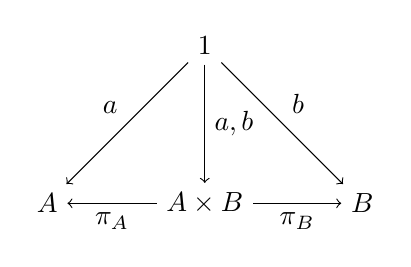
\begin{tikzpicture}[auto]
				\node (a) at (0, 0) {$A$};
				\node (b) at (4, 0) {$B$};
				\node (ab) at (2, 0) {$A\times B$};
				\node (x) at (2, 2) {$1$};
				\draw[->] (ab) to node {$\pi_A$}(a);
				\draw[->] (ab) to node[swap] {$\pi_B$}(b);
				\draw[->] (x) to node[swap] {$a$}(a);
				\draw[->] (x) to node {$b$}(b);
				\draw[->] (x) to node {$\tuple{a,b}$}(ab);
			\end{tikzpicture}
		\end{center}
	\end{proof}
	\begin{proof}[$\Longleftarrow$]
		限定的ではあるが、まずは任意の対象$X$に終対象$1$を当てはめた場合を見ていき、その後任意の対象$X$に拡張する。
		射影射となる射影写像$\pi_A,\pi_B$を任意の順序対$\tuple{a,b}$において\[\pi_A(\tuple{a,b})=a,\ \pi_B(\tuple{a,b})=b\]と定義する。

		直積集合の定義より、任意の元$a$、$b$に対して順序対$\tuple{a,b}$が存在し、順序対ではない元や重複する元を含まないことから、積の普遍性を部分的に満たすことがわかる。
		\begin{center}
			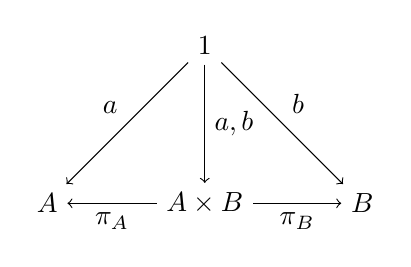
\begin{tikzpicture}[auto]
				\node (a) at (0, 0) {$A$};
				\node (b) at (4, 0) {$B$};
				\node (ab) at (2, 0) {$A\times B$};
				\node (x) at (2, 2) {$1$};
				\draw[->] (ab) to node {$\pi_A$}(a);
				\draw[->] (ab) to node[swap] {$\pi_B$}(b);
				\draw[->] (x) to node[swap] {$a$}(a);
				\draw[->] (x) to node {$b$}(b);
				\draw[->] (x) to node {$\tuple{a,b}$}(ab);
			\end{tikzpicture}
		\end{center}
		次に元の対から写像の対に拡張して考える。写像の対が一意に存在することを元の対が一意に存在することから示せばよい。

		写像$\mor{f}{X}{A}$と写像$\mor{g}{X}{B}$の写像の対$\tuple{f,g}$を$X$の任意の元$x$に対して\[\tuple{f,g}(x)=\tuple{f(x),g(x)}\]と定義する。

		また、
		\begin{align*}
			(\pi_A\circ\tuple{f,g})(x)&=\pi_A(\tuple{f,g}(x))&\text{(写像の合成の定義)}\\
			&=\pi_A(\tuple{f(x),g(x)})&\text{(写像の対の定義)}\\
			&=f(x)&\text{(元の対の可換性)}\\
			(\pi_B\circ\tuple{f,g})(x)&=\pi_B(\tuple{f,g}(x))&\text{(写像の合成の定義)}\\
			&=\pi_B(\tuple{f(x),g(x)})&\text{(写像の対の定義)}\\
			&=g(x)&\text{(元の対の可換性)}
		\end{align*}
		よって\[\pi_A\circ\tuple{f,g}=f,\ \pi_B\circ\tuple{f,g}=g\]が成り立つから写像の対は射の対としての可換性を満たすことがわかる。
		またこのような射の対は$\mor{f}{X}{A}$、$\mor{g}{X}{B}$なる任意の二射$f,g$に対し存在する。

		仮に$\pi_A\circ h=f,\ \pi_B\circ h=g$となる射$\mor{h}{X}{A\times B}$が存在しても、
		$\pi_A(h(x))=f(x),\ \pi_B(h(x))=g(x)$と元の対の一意性より$h(x)=\tuple{f(x),g(x)}$が成り立ち$h=\tuple{f,g}$となる。よって写像$f,g$の写像の対$\tuple{f,g}$は一意に存在する。
		\begin{center}
			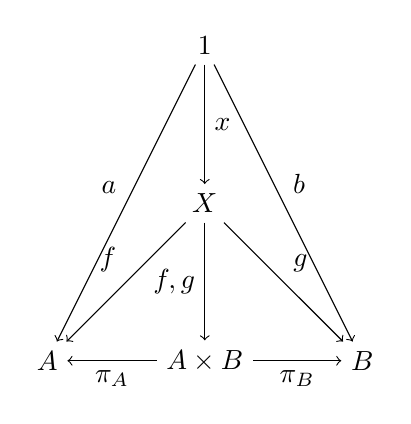
\begin{tikzpicture}[auto]
				\node (a) at (0, 0) {$A$};
				\node (b) at (4, 0) {$B$};
				\node (ab) at (2, 0) {$A\times B$};
				\node (i) at (2, 4) {$1$};
				\node (x) at (2, 2) {$X$};
				\draw[->] (ab) to node {$\pi_A$}(a);
				\draw[->] (ab) to node[swap] {$\pi_B$}(b);
				\draw[->] (x) to node[swap] {$f$}(a);
				\draw[->] (x) to node {$g$}(b);
				\draw[->] (x) to node[swap] {$\tuple{f,g}$}(ab);
				\draw[->] (i) to node[swap] {$a$}(a);
				\draw[->] (i) to node {$b$}(b);
				\draw[->] (i) to node {$x$}(x);
			\end{tikzpicture}
		\end{center}
	\end{proof}
	